\PassOptionsToPackage{unicode}{hyperref}
\documentclass[20pt]{beamer}
%\documentclass[t]{beamer}

\usepackage[
  orientation=portrait,
  size=a0,
  scale=1.0,
]{beamerposter}

\usetheme{tudoposter}

\usepackage{fontspec}

\usepackage{polyglossia}
\setmainlanguage{german}

\usepackage{csquotes}
\usepackage{microtype}
\usepackage{mathtools}

\usepackage{blindtext}

\usepackage{multicol}
\setlength{\columnsep}{1em}

\usepackage{graphicx}

\usepackage[
  locale=DE,                   % deutsche Einstellungen
  separate-uncertainty=true,   % Immer Fehler mit \pm
  per-mode=symbol-or-fraction, % m/s im Text, sonst Brüche
  output-decimal-marker=.      % Punkt statt Komma
]{siunitx}
%% this is used to create an inline bibliography
\usepackage[backend=biber, style=numeric]{biblatex}
\addbibresource{biblatex-phys.bib}

\DeclareFieldFormat*{title}{\textit{#1}}
\renewcommand*{\bibfont}{\footnotesize}
\defbibenvironment{bibliography}
  {\noindent}
  {\unspace}
  {}


\renewbibmacro*{begentry}{%
  \usebeamercolor{bibliography item}%
  \color{bibliography item.fg}%
  \printtext[labelnumberwidth]{%
    \printfield{prefixnumber}%
    \printfield{labelnumber}%
  }%
  \setunit{\addnbspace}%
}
\renewcommand*{\finentrypunct}{\addperiod\space}

\newlength{\thirdtextwidth}
\setlength\thirdtextwidth{0.333333\textwidth}


\title{Lehrstuhlversuch zur Thermolumineszenzdosimetrie}
\author{Alexander Droßel, Philipp Hoffmann, Robert Theinert}
\date{Wintersemester 2016/17}

\titlegraphic{%
  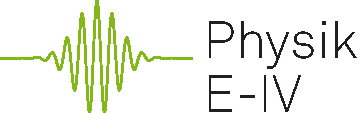
\includegraphics[width=0.6\linewidth]{Physik-E4-Logo}
}
\institute{%
  
\includegraphics[width=0.9\linewidth]{tudo.pdf}%
}

\begin{document}
  \begin{columns}[onlytextwidth]%

    \begin{column}{0.5\textwidth}%
      \begin{block}[equal height group=A]{Einleitung}%
              \begin{multicols}{2}
				\begin{figure}
            		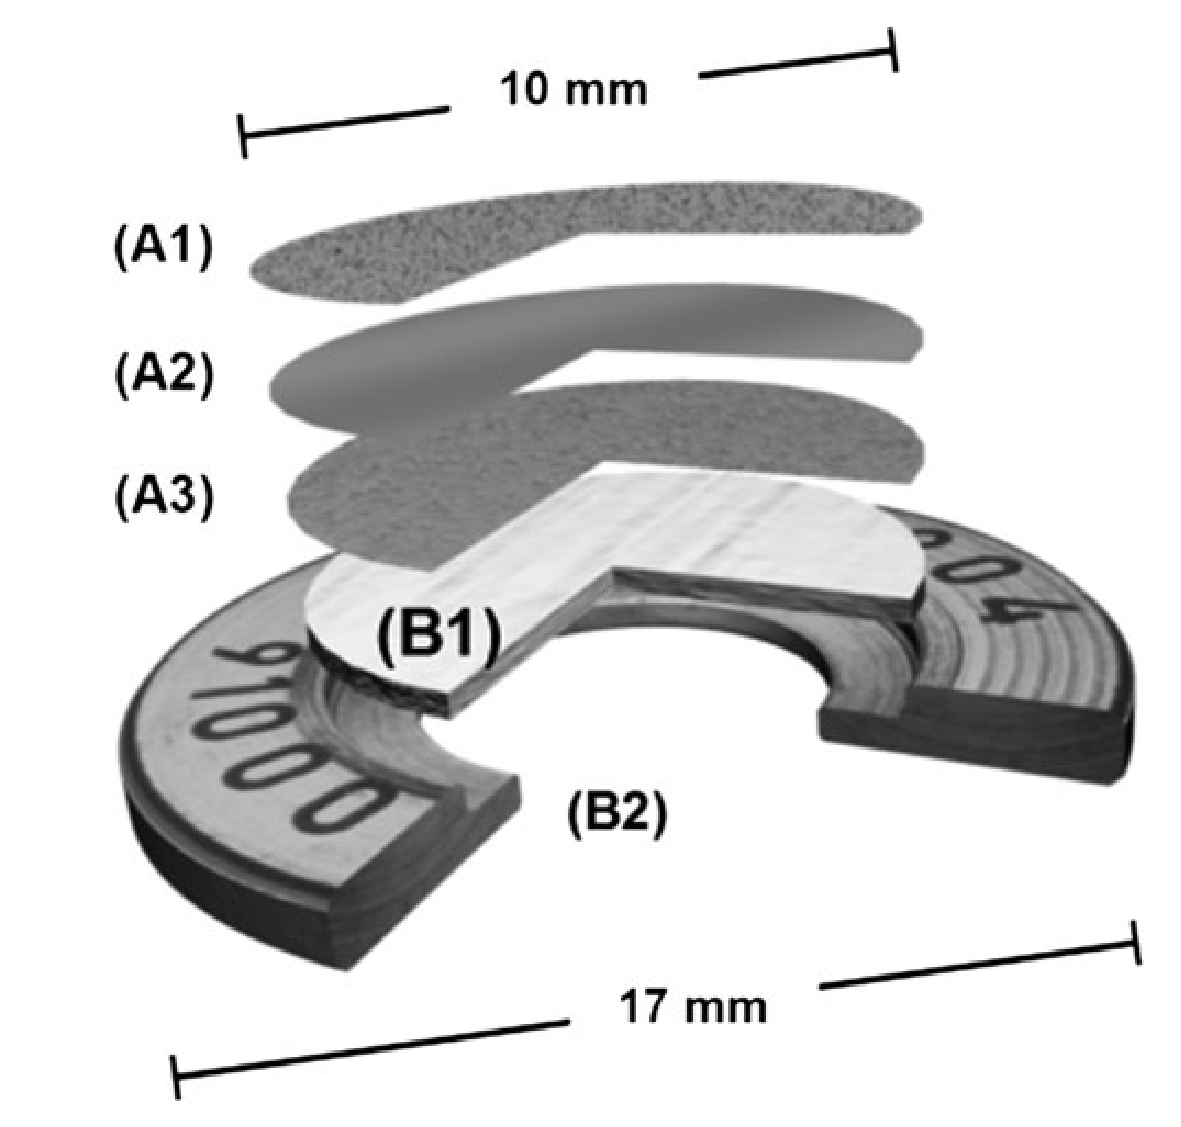
\includegraphics[width=0.8\linewidth]{bilder/dosi}\\
                    \caption{Aufbau eines Dünnschicht-Thermolumineszenzdosimeters.\cite{TL-DOS} }
            		\label{TL-DOS}
          		\end{figure}
                  %\columnbreak
                  \begin{large}
          Um Personen, die in ihrer Arbeit kontinuierlich Strahlung ausgesetzt sind, amtlich zu überwachen, werden Dosimeter verwendet.
          Die zurzeit in der Testphase befindlichen TL-DOS Dosimeter (siehe Abbildung \ref{TL-DOS}) werden am Materialprüfungsamt NRW ausgelesen, wodurch sich ein Rückschluss darauf ziehen lässt, welcher Strahlendosis eine Person ausgesetzt war und ob diese den gängigen Richtwert überschreitet. Nach der Testphase sollen sie als Ganzkörperdosimeter verwendet werden.
                  \end{large}

                  \begin{large}
                      Die TL-DOS Dosimeter basieren auf dem Prinzip der Thermolumineszenz. Das Dosimeter besteht aus 5 Schichten: der aktiven Schicht (A1), der reflektiven Schicht (A2), der Keramik-Schicht zur Hintergrundminimierung (A3) und der Carrier-Schicht (B1). Ziel dieses Versuchs ist es anhand von Messreihen der Thermolumineszenz von Dosimetern mit bekannter Bestrahlungsdosis eine Methode zu entwickeln, die es erlaubt Dosimeter, die einer unbekannten Strahlungsdosis ausgesetzt wurden, zu analysieren. 
          %und einem "Codering" (B2) zum befestigen der verschiedenen Schichten.
                  \end{large}
        \end{multicols}      
      \end{block}%
    \end{column}%
    \begin{column}{0.5\textwidth}%
      \begin{block}[equal height group=A]{Theoretische Grundlagen zur Thermolumineszenz}%
        \begin{multicols}{2}
          \begin{figure}
            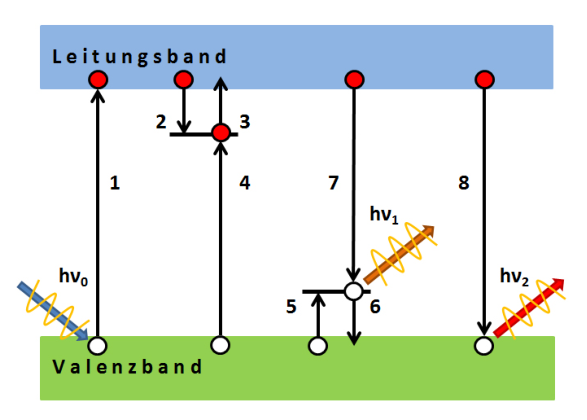
\includegraphics[width=\linewidth]{bilder/gap}\\
            \caption{Schema zur Bandlücke mit den darin befindlichen Traps. \cite{gap} }
            \label{gap}
          \end{figure}
          %\columnbreak
                  \begin{large}
          Im Dosimeter wird LiF:Mg,Ti als aktives Medium verwendet, also Lithiumfluorid mit Magnesium und Titan Dotierung. Lithiumfluorid weißt eine Bandlücke von $\SI{13.27}{eV}$ auf; mittels der Dotierung durch Mg und Ti entstehen in der Bandlücke sogenannte Traps. Die Traps können durch Strahlung angeregte Elektronen einfangen. Je nach Abstand zum Valenzband benötigen die Elektronen unterschiedlich viel Energie um dorthin zurückzugelangen, zur Veranschaulichung siehe Abbildung \ref{gap}. Dies geschieht je nach Trap mit einer unterschiedlichen Halbwertszeit. Dieser Vorgang kann beschleunigt werden, indem dem Material Wärmeenergie zugeführt wird, wodurch die Elektronen die nötige Energie für einen Wechsel der Bänder erhalten. Geschieht dies, rekombiniert das Elektron mit einem hinterlassenen Loch und erzeugt dabei ein Photon. Die beim Aufheizen des Materials entstehenden Photonen stehen somit in einem direkten Zusammenhang zu der absorbierten Strahlung.
                  \end{large}
        \end{multicols}
      \end{block}%
    \end{column}%
    %\begin{column}{0.5\textwidth}%
      %\begin{alertblock}[equal height group=A]{Test}%
        %\begin{multicols}{2}
          %\blindtext
          %\blindtext
        %\end{multicols}
      %\end{alertblock}%
    %\end{column}%
  \end{columns}%

  \begin{columns}[t, onlytextwidth]%
    \begin{column}{0.666\textwidth}%
      \begin{block}{Auswerten der Glühkurve}%
              \begin{multicols}{2}
                  \begin{large}
                  Beim Auswerten des Dosimeters wird es erhitzt.
                  Dadurch werden die Elektronen aus den Traps gelöst und es werden Photonen erzeugt, die detektiert werden.
                  Wird die Zahl der so erzeugten Photonen gegen die Zeit aufgetragen ergibt sich eine Glühkurve, wie sie in Abbildung~\ref{pic:Glühkurve} zu sehen ist. 
                  Die Materialzusammensetzung des TL-DOS Dosimeters sorgt für vier Peaks in der Kurve. 
          Diese entstehen durch die verschiedenen Energien, die nötig sind um die Elektronen aus den jeweiligen Traps auszulösen. 
                  \end{large}

                  \begin{large}
Für diesen Versuch besonders wichtig ist das Integral der beim Erhitzen des Dosimeters detektierten Photoelektronen, da es im besonders direkten Zusammenhang zu der vom Dosimeter aufgenommenen Strahlung, der Dosis, steht.
Andere mit der Dosis korrelierte Attribute sind die durchschnittliche Anzahl der Photoelektronen vor und nach dem Heizvorgang und dessen Start- und Endzeitpunkt, als auch die Höhen von an die Glühkurve gefitteten Gaussfunktionen.
          Diese und weitere Attribute sind in Abbildung~\ref{pic:Glühkurve} eingezeichnet.
                  \end{large}
          \begin{figure}
              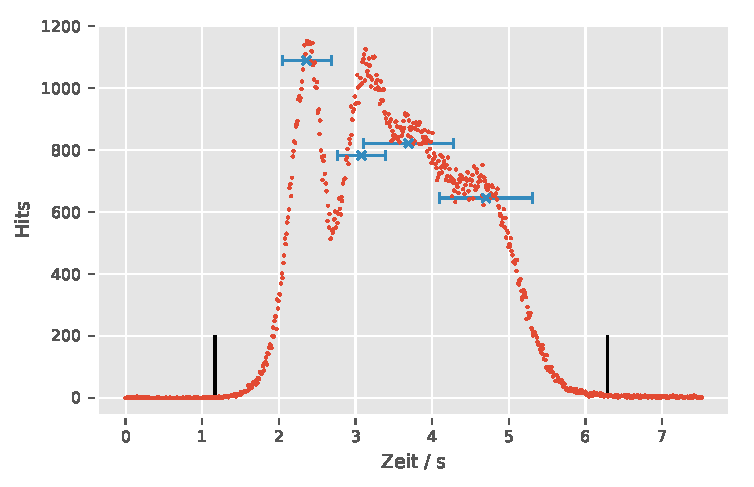
\includegraphics[width=\linewidth]{./python/attributeVisualization}
              \caption{Glühkurve nach einer Bestrahlungsdosis von \SI{5}{mSv} mit einigen generierten Attributen. Die Vertikalen Linien zeichnen Start- und Endpunkt des Heizvorgangs aus. Die blauen Markierungen sind die Mittelwerte und Breiten der an die Glühkurve gefitteten Gaussfunktionen.}
              \label{pic:Glühkurve}
          \end{figure}
          \columnbreak

                  \begin{large}
          In Abbildung~\ref{attrdiff} sind die Attributsverteilungen von einigen Attributen zu sehen, die untereinander eine Pearson Korrelation kleiner 0.2 haben und eine Trennung von unterschiedlichen Dosen ermöglichen.
                      Um eine hohe Genauigkeit zu erreichen wird anhand dieser und anderer Attribute eine Regression mittels des RandomForest-Algorithmus, implementiert in Scikit-Learn~\cite{sklearn} durchgeführt. 
                      %
                  Hierbei wird ein Random Forest (RF) auf einen Satz gegebener Glühkurven mit bekannter Dosis trainiert.
                  \end{large}

                  \begin{large}
                  Der RF erstellt Entscheidungsbäume, in denen an jedem Knoten Schnitte in einem Attribut durchgeführt werden. Für jeden Schnitt wird die quadrierte Abweichung im Bezug auf die Kalibrierungsdosis minimiert. Die gemittelte Dosis der Ereignisse, die im letzten Knoten des Baumes liegen, ist die Vorhersage des Baumes für Ereignisse mit der jeweiligen Kombination an Attributsschnitten. Anschließend werden die Vorhersagen aller Bäume gemittelt.
          Der RF kann nun die Dosen von unbekannten Glühkurven vorhersagen.
          %
                  \end{large}
          %\columnbreak
          \begin{figure}
              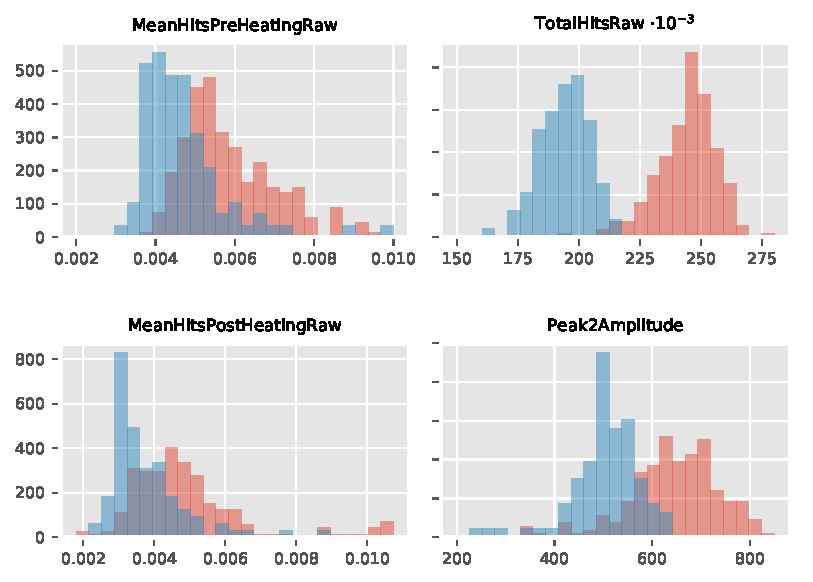
\includegraphics[width=\linewidth]{./python/attrDiff.pdf}
              \caption{Normierte Histogramme von vier generierten Attributen von Kalibrierungsmessung mit \SI{4}{mSv} (blau) \SI{5}{mSv} (rot).}
              \label{attrdiff}
          \end{figure}
              \end{multicols}
      \end{block}%
        %
      \begin{block}{Zusammenfassung}%
          \begin{multicols}{2}
                  \begin{large}
          Es zeigt sich, dass die Vorhersage der Dosen mit einem Random Forest möglich ist.
          Die Richtwerte für das maximale mittlere Überschätzen der Dosis von 18\% und dem maximalen Unterschätzen der Dosis von 13\% werden eingehalten.
          Die Werte liegen bei 6.0\% und 8.4\%.
                  \end{large}

                  \begin{large}
                  Die Genauigkeiten des RF lassen sich jedoch in zwei Bereiche einteilen und weisen auf Übertraining hin.
                      Unter $\SI{0.2}{mSv}$ sind die mittleren Abweichungen mit etwa 6\% groß und die geschätzten Dosen streuen kontinuierlich. In Abbildung~\ref{scatter1} ist dieser Dosisbereich in einem Scatterplot dargestellt. 
                  \end{large}

                  \begin{large}
                      Über $\SI{0.1}{mSv}$ liegen die Dosiswerte so weit auseinander, dass der RF keine kontinuierliche Regression durchführt, sondern die Glühkurven nur noch in den stark diskreten Kalibrierungsdosen zuordnet. Dies kann unterbunden werden indem die Dosen randomisiert werden und der Parameterraum damit kontinuierlicher ausgefüllt wird. Allgemein sollte eine höhere Anzahl an Kalibrierungsdosen, die mit 1426 für ein multivariates Verfahren aktuell noch recht gering ist, zu einer genaueren Regression des RF führen.
                  \end{large}

                  \begin{large}
            %Die großen Unterschiede in der Regressionsqualität für die verschiedenen Dosisbereiche, weisen jedoch auf Übertraining hin und es sollten noch mehr und randomisierte Kalibrierungsdosen aufgenommen werden, bevor so eine Multivariate Methode für das Auswerten der Dosimeter im täglichen Gebrauch verwendet werden kann.
              %Es ist nicht bekannt, ob die Dosen mit den größten Abweichungen mit anderen Methoden besser vorhergesagt werden können.können in einer kombinierten Auswertung können in einer kombinierten Auswertung 
              %Sollte das der Fall sein, können in einer kombinierten Auswertung 
                  \end{large}
                      
                  \begin{large}
            Attribute, die die Fertigungsstreuung der Dosimeter beschreiben, sollten die Regression verbessern.
            Es ist aber bereits möglich das Verfahren alleine oder in Kombination mit einem einfacheren Schätzer zu verwenden.
                  \end{large}
          \begin{figure}
              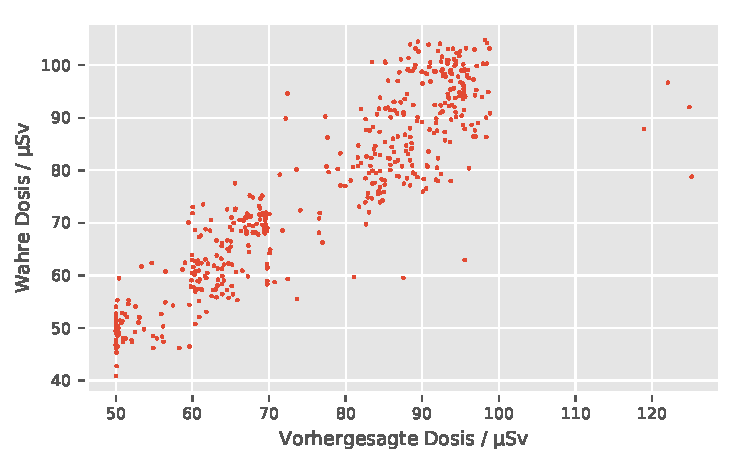
\includegraphics[width=\linewidth]{./python/scatter.pdf}
              \caption{Scatterplot der wahren und vorhergesagten Dosen. Zur Besseren Unterscheidung der Wertepaare wurde auf die wahren Dosen ein gauss'sches Rauschen mit $ \mu = 0$ und $\sigma = \SI{3}{µSv}$ addiert.}
              \label{scatter1}
          \end{figure}
          \end{multicols}
      \end{block}%
  \begin{block}[equal height group=bottom, fonttitle=\normalsize]{Referenzen}
      \nocite{*}\footnotesize%
      \printbibliography%
  \end{block}

    \end{column}

    \begin{column}{0.333\textwidth}%
      %\begin{block}[equal height group=A]{Auswertung der Regression}%
      \begin{block}{Auswertung der Regression}%
              %\begin{multicols}{1}
                  \begin{large}
            Zum Training des RF werden insgesamt 1426 Glühkurven mit 16 diskreten Dosen im Bereich von $\SI{0.05}{mSv}$ bis $\SI{10}{mSv}$ verwendet. Es wird eine fünffache Kreuzvalidierung durchgeführt, so dass in jedem Schritt 80\% der Kalibrierungsdosen zum Training und 20\% der Dosen zum Testen der Vorhersage verwendet werden. So kann für alle vorhandenen Dosen eine Überprüfung der Genauigkeit der Regression vorgenommen werden. 
                  \end{large}

                  \begin{large}
                  In Abbildung~\ref{absAbw} sind die absoluten Abweichungen der Vorhersagen des RF gegenüber den wahren Werten der Dosis histogrammiert. Die Verteilung hat ihr Maximum nahe $\SI{0.0}{µSv}$ und ist sehr schmal. 
                  \end{large}

                  \begin{large}
                  Das Mittel der Beträge der relativen Abweichungen ist 0.4\%. In Abbildung~\ref{boxplot} sind ihre Verteilungen für alle vorhandenen Werte an Kalibrierungsdosen dargestellt. Es ist zu sehen, dass die Abweichungen für Dosen größer $\SI{0.1}{mSv}$ gegen Null gehen. Die Abweichungen für Werte unter $\SI{0.2}{mSv}$ sind deutlich größer als 1\%, mit einem Mittelwert von 6.4\%. 
                     Wird ein neuer RF ausschließlich auf Dosen kleiner $\SI{0.2}{mSv}$ trainiert, lassen sich diese Abweichungen auf 6.0\% reduzieren. 
                  \end{large}

          \begin{figure}
              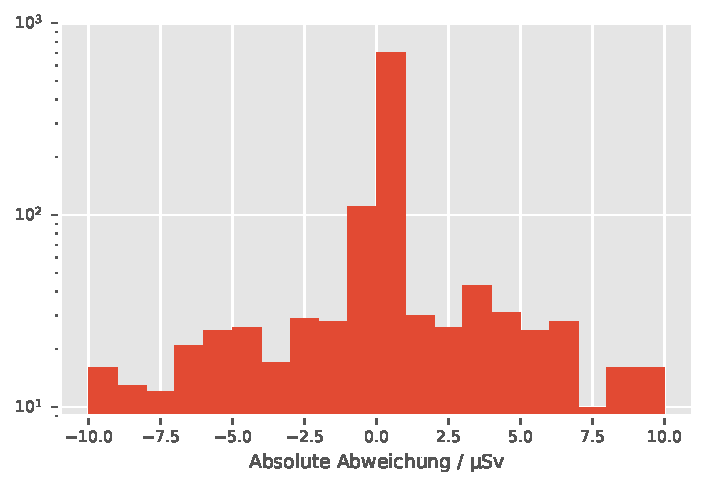
\includegraphics[width=\linewidth]{./python/absAbweichung.pdf}
              %\vspace{-1.0em}
              \caption{Histogramm der absoluten Abweichungen zwischen ermittelter und wahrer Dosis.}
              \label{absAbw}
          \end{figure}
          \begin{figure}
              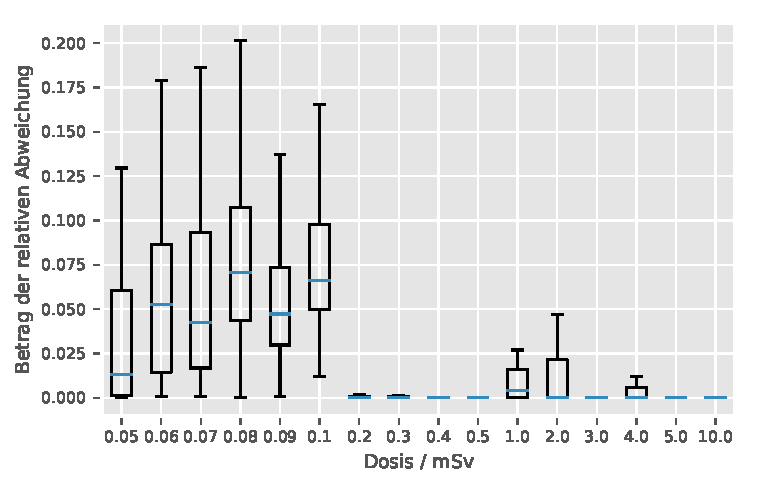
\includegraphics[width=\linewidth]{./python/boxplot}
              %\vspace{-0.5em}
              \caption{Boxplots der relativen Abweichungen zwischen vorhergesagten und wahren Dosen für 1426 Kalibrierungsdosen. Die blauen Balken kennzeichnen den Mittelwert, die Box ihre Standardabweichung. 
              Die schwarzen Balken zeigen den größten und kleinsten Wert der Verteilung.
              }
              \label{boxplot}
          \end{figure}
              %\end{multicols}
      \end{block}%

  %\begin{block}

    \end{column}%


  \end{columns}%



  %\begin{columns}[c, onlytextwidth]%
    %\begin{column}{0.33\textwidth}%
      %%\begin{block}{Zusammenfassung}%
  %\begin{block}[equal height group=bottom, fonttitle=\normalsize]{Referenzen}
      %\nocite{*}\footnotesize%
      %\printbibliography%
  %\end{block}
    %\end{column}%
  %\end{columns}


  %\vspace*{\fill}
  %\begin{block}[equal height group=bottom, fonttitle=\normalsize]{Referenzen}
    %%\begin{multicols}{3}
      %\nocite{*}\footnotesize%
      %\printbibliography%
    %%\end{multicols}
  %\end{block}
\end{document}
